\section{Memory Transaction Optimization}
\label{sec:strategies}
{\color{red}We take the 2D convolution shown in Figure \ref{fig:twostrategies} as an example to demonstrate how to optimize convolution operations.}
%As a motivation example, consider Figure \ref{fig:twostrategies} that shows a simple 2D convolution executing on a GPU.
Here, we slide a $5 \times 5$ filter over a $6 \times 11$ image to produce a $2 \times 7$ output. In this example, each thread calculates one column of the output. For example, threads 0 and 1 could execute code to slide the filter along the width dimension. Both threads load two overlapped regions from the input image, thereby generating four duplicate columns. Assume thread 6 demonstrates the process of sliding the filter along the height dimension. It loads two overlapped regions and generates four duplicate rows.

%Our approach can eliminate redundant elements on the column and the width dimensions to reduce the number of memory accesses.  In the proposed column reuse algorithm, we let each thread load the required first and last columns and retrieve the remaining from other threads through shuffle instructions. The difference in the usage of shuffle instructions between our algorithms and the previous study \cite{vasilache2014fast} is discussed in Section \ref{sec:strategies}. In the proposed row reuse algorithm, we let each thread load overlapped rows only once and multiply each row with multiple rows of a filter to calculate multiple output elements. A major performance issue encountered in our implementation is that the thread local arrays with dynamic indexing are placed in the local memory, which possesses the same access latency as the global memory. To solve this problem, we use pack and unpack operations to transform dynamic indexing into static indexing.

Our approach optimizes convolution operations on GPUs by reusing column and row elements. Before getting to details, we first give the notations used in the remaining chapters in Table \ref{tab:notations}.

\begin{table}[t!]
\caption{Notations for the convolution operation.}
	\begin{tabular}{c|c}
	\hline
		$I$, $F$, $O$ & Input, Filter, Output \\
		\hline
		$N$, $C$, $H$, $W$ & batch size, channel, height, width\\
		\hline
	\end{tabular}
	\label{tab:notations}
\end{table}

%In this paper, we use $I$, $F$ and $O$ to denote an input, a filter and an output tensor respectively. Each tensor is indexed according to its batch size ($N$), channel ($C$), height ($H$) and width ($W$). For example, $I_N$, $I_C$, $I_H$ and $I_W$ represent the batch size, number of channels, width and height of an input, $I$.

\subsection{Column Reuse}
\label{sec:creuse}
\begin{figure*}[t!]
	\begin{subfigure}{0.33\textwidth}
		\centering
		\captionsetup{width=0.9\textwidth}
		 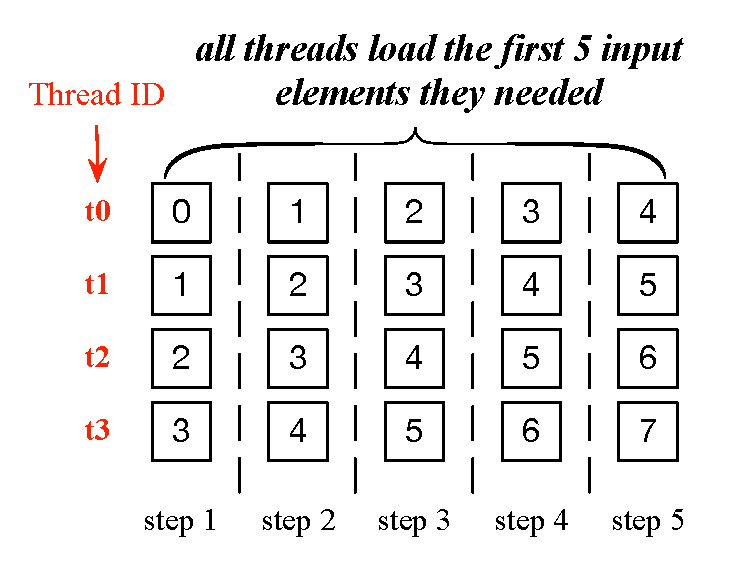
\includegraphics[width=0.98\textwidth,height=4.5cm]{./figure/directconv.eps}
		 \caption{Direct convolution: Each thread loads 5 input elements from global memory.}
		 \label{fig:directalgo}
	\end{subfigure}
	\begin{subfigure}{0.3\textwidth}
		\centering
		\captionsetup{width=0.9\textwidth}
		 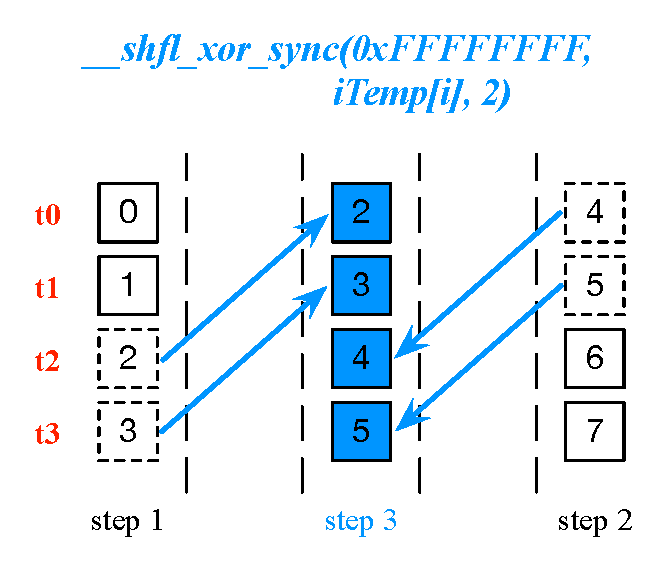
\includegraphics[width=\textwidth,height=4.5cm]{./figure/optalgo1.eps}
		 \caption{Optimized convolution: each thread retrieve its third element from the corresponding thread.}
		 \label{fig:optalgo1}
	\end{subfigure}
	\begin{subfigure}{0.3\textwidth}
		\centering
		\captionsetup{width=0.9\textwidth}

		 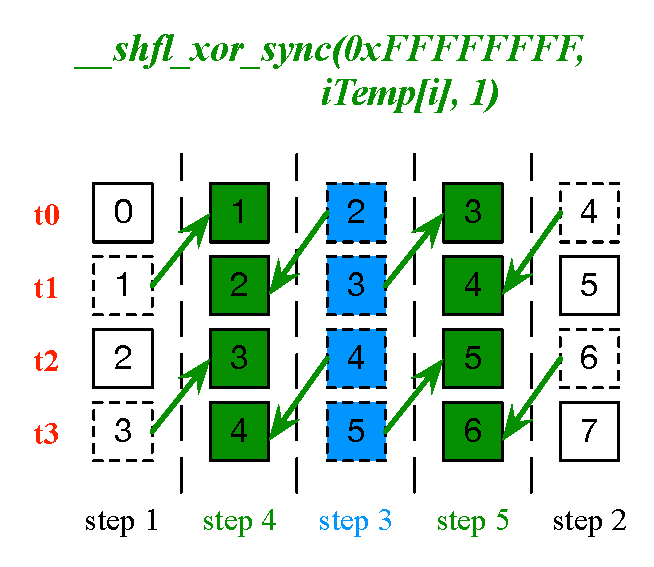
\includegraphics[width=0.96\textwidth,height=4.5cm]{./figure/optalgo2.eps}
		 \caption{Optimized convolution: each thread retrieve its second and fourth elements from corresponding threads.}
		 \label{fig:optalgo2}
	\end{subfigure}
  \caption{Illustration of direct and optimized convolution. We use a $5 \times 5$ filter  and each thread calculate convolution for one output element. Here we demonstrate how each thread processes first 5 corresponding input elements.}
   \label{fig:corealgo}
\end{figure*}



Figure \ref{fig:corealgo} depicts our column reuse algorithm, which consists of a number of step.

 In step 1 of Figure \ref{fig:directalgo}, each thread loads the first corresponding input elements from the
global memory. Given that the addresses of these elements are contiguous (0, 1, 2, 3), the memory controller can coalesce the accesses into
one memory transaction. Therefore, five memory transactions are required for steps 1-5 of. Each pair of adjacent threads have four
duplicate input elements, which corresponds to the duplicate columns in Figure \ref{fig:twostrategies}.

The input elements 1, 2 and 3 loaded in step 2 would have already been loaded by threads $t1$, $t2$ and $t3$ in step 1 (Figure
\ref{fig:directalgo}). Therefore, we can retrieve the input elements 1, 2 and 3 from the threads $t1$, $t2$ and $t3$ instead of loading
them from the global memory (or L1 cache). This kind of duplication also occurs in steps 3, 4 and 5.

To eliminate the redundant loads, we use the shuffle instructions to exchange input elements among different threads. In steps 1
and 2 of Figure \ref{fig:optalgo1}, each thread loads the corresponding first and fifth input elements from the global memory. In step 3, each
thread utilizes the shuffle instruction to retrieve the third element from another thread. Threads $t0$ and $t1$ retrieve the third elements
from threads $t2$ and $t3$, respectively, and provide the fifth elements (dashed squares in step 2) for both threads.
Similarly, threads $t2$ and $t3$ retrieve the third elements from threads $t0$ and $t1$, respectively, and provide the first
elements (dashed squares in step 1) for threads $t0$ and $t1$. This exchange process can be implemented using the instruction
$shfl\_xor(iTemp[i],2)$ (taking CUDA shuffle as an example, \cite{CUDAtoolkit} provides the exact form of the shuffle instructions), where $iTemp$ is the thread local
array used to store the five input elements, and $i$ indexes which element to provide. For threads $t0$ and $t1$, both need to provide the fifth
elements, thus $i=4$. For threads $t2$ and $t3$, both need to provide the first elements, thus $i=0$. The procedure presented in Figure  \ref{fig:optalgo2} is the same as that in Figure \ref{fig:optalgo1}, except that each thread in Figure 3c retrieve itsthe former retrieves the second and fourth elements from its neighboring threads.

However, the instruction $shfl\_xor(iTemp[i],2)$ significantly degrades the performance of the convolution because $iTemp$ is an array with
dynamic indexing, which means that the compiler cannot decide which element to provide at the compile time. Therefore, the compiler
places array $iTemp$ in the local memory, which possesses the same access latency as the global memory, instead of the registers. This process significantly increases the memory access time and degrades the performance of the convolution.

\begin{figure}[t!]
	\centering
	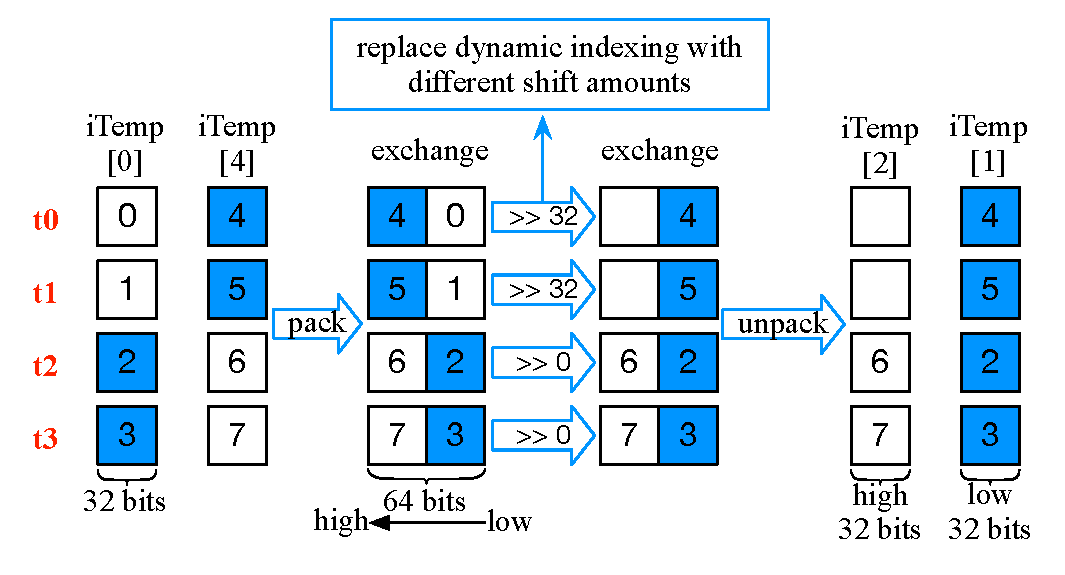
\includegraphics[width=\columnwidth,height=4.5cm]{./figure/exchange.eps}
\caption{Convert the dynamic indexing of array $iTemp$ into static indexing. Therefore, The compiler can put $iTemp$ into registers instead of local memory.}
\label{fig:exchange}
\end{figure}


\begin{algorithm}[t!]
	$tid \gets threadIdx.x$\;
	$iTemp[0] \gets iData[iIndex]$\;
	$iTemp[4] \gets iData[iIndex+4]$\;
	$mov\ exchange, \{iTemp[0], iTemp[4]\}$\;
	$shift \gets ((tid+2)\&2)<<4$\;
	$exchange \gets exchange >> shift$\;
	$mov\ \{iTemp[1],iTemp[2]\}, exchange$\;
	$iTemp[2] \gets shfl\_xor(iTemp[1],2)$\;	
	
	\caption{Data exchange algorithm for retrieving the third element}
	\label{algo:basic}
\end{algorithm}

To convert dynamic indexing into static one, we design Algorithm \ref{algo:basic} for step 3 in Figure \ref{fig:optalgo1} and
Algorithm \ref{algo:basic2} for steps 4 and 5 in Figure \ref{fig:optalgo2}. Both algorithms use the same method but deal with different
situations. Moreover, both algorithms can change dynamic indexing into static indexing and reduce the number of memory accesses. We then use Algorithm
\ref{algo:basic} as an example to illustrate the elimination of dynamic indexing.

Figure \ref{fig:exchange} illustrates the process of Lines 4-7 of Algorithm \ref{algo:basic}. First, each thread loads the corresponding first and fifth input elements into $iTemp$ (Lines 2-3). Second, the 32-bit elements are packed into a 64-bit variable $exchange$, where $iTemp[4]$ and $iTemp[0]$ are the high and low 32 bits, respectively (Line 4). The exchange is right-shifted by 32 to place $iTemp[4]$ in the low 32 bits because threads $t0$ and $t1$ must provide the fifth
elements, which are the high 32 bits of $exchange$. Threads $t2$ and $t3$ must provide the first elements, which are already the low 32 bits of $exchange$. Therefore, we right shift $exchange$ in threads $t2$ and $t3$ by 0. The shift amounts of each thread is calculated on the basis of the thread ID (Line 5). Third, unpack $exchange$ into $iTemp[2]$
(high 32 bits) and $iTemp[1]$ (low 32 bits) (Line 7). And $iTemp[1]$ is the element that each thread must provide. Lastly, the
shuffle instruction is used to exchange the elements among the threads (Line 8).

In contrast to the previous usage of shuffle instructions \cite{vasilache2014fast}, Algorithm \ref{algo:basic} successfully replace dynamic
indexing $i$ in $shfl\_xor(iTemp[i],2)$ with static indexing $1$ in $shfl\_xor(iTemp[1],2)$. Algorithm \ref{algo:basic} successfully
eliminates dynamic indexing and therefore all thread local variables can be put in registers, which significantly improve the performance
of convolution.

\begin{algorithm}[t!]
	$tid \gets threadIdx.x$\;
	$mov\ exchange, \{iTemp[0], iTemp[2]\}$\;
	$shift \gets ((tid+1)\&1)<<5$\;
	$exchange \gets exchange >> shift$\;
	$mov\ \{iTemp[0],iTemp[1]\}, exchange$\;
	$iTemp[1] \gets shfl\_xor(iTemp[0],1)$\;	
	\caption{Data exchange algorithm for retrieving the second element}
	\label{algo:basic2}
\end{algorithm}

Steps 4 and 5 in Figure \ref{fig:optalgo2} have similar procedure as step 3 in Figure \ref{fig:optalgo1}. Thus, we slightly modify
Algorithm \ref{algo:basic} to obtain Algorithm \ref{algo:basic2}. The main distinction between the two algorithms is that four threads are involved to exchange the
elements in Figure \ref{fig:optalgo1}, whereas only two adjacent threads are involved in Figure \ref{fig:optalgo2}. Therefore, the shift amounts for each thread (Line 3) should be recalculated, and the arguments of the shuffle instruction (Line 6) should be changed.

In summary, Algorithms \ref{algo:basic} and \ref{algo:basic2} can reduce the number of memory transactions from 5 to 2 and 25 to 10 when 5 and 25 input elements are loaded, respectively. This reduction greatly improves the performance of the convolution.

\subsection{Row Reuse}
\label{sec:rowreuse}
\begin{figure}
	\centering
	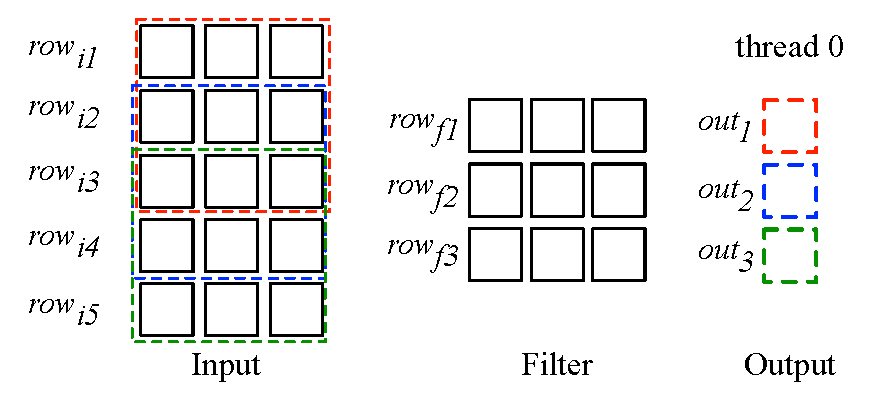
\includegraphics[width=\columnwidth,height=3.7cm]{./figure/rowreuse.eps}
\caption{A $3 \times 3$ filter is used to slide over the input image along height dimension and produce a column of output elements. One thread is used to calculate this column of output elements.}
\label{fig:rowreuse}
\end{figure}

Figure \ref{fig:rowreuse} shows that when sliding the filter over the input image along the height dimension, we can obtain a column of the output elements. Our design then uses one thread to calculate one column of the output elements. Based on Figure \ref{fig:rowreuse},
we can perform convolution as follows:

\begin{gather*}
  out_1=row_{i1} \cdot row_{f1} + row_{i2} \cdot row_{f2} + row_{i3} \cdot row_{f3} \\
out_{2}=row_{i2} \cdot row_{f1} + row_{i3} \cdot row_{f2} + row_{i4} \cdot row_{f3} \\
	out_{3}=row_{i3} \cdot row_{f1} + row_{i4} \cdot row_{f2} + row_{i5} \cdot row_{f3}
\end{gather*}

The above equations suggest that $row_{i2}$ and $row_{i4}$ are loaded twice, and $row_{i3}$ is loaded three times; nice rows should be loaded in total. To eliminate row duplications, we redesign the execution of the convolution. After loading a row from the input, we determine the number of output elements that need the row. For example, $out_1$ needs $row_{i1}$, and $out_1$ and $out_2$ need $row_{i2}$. Then, we use
this row to do inner product with corresponding rows of the filter to calculate the output elements that this row. The resigned formulations are shown as follows:
\begin{equation}\nonumber
\begin{aligned}
load\ row_{i1}:
&\ out_1=row_{i1} \cdot row_{f1} \\
load\ row_{i2}:
&\ out_1 = out_1+row_{i2} \cdot row_{f2}\\
&\ out_2=row_{i2} \cdot row_{f1}\\
load\ row_{i3}:
&\ out_1 = out_1+row_{i3} \cdot row_{f3}\\
&\ out_2 = out_2+row_{i3} \cdot row_{f2}\\
&\ out_{3}=row_{i3} \cdot row_{f1}\\
load\ row_{i4}:
&\ out_2=out_2+row_{i4} \cdot row_{f3} \\
&\ out_3=out_3+row_{i4} \cdot row_{f2}\\
load\ row_{i5}:
&\ out_3=out_3+row_{i5} \cdot row_{f3}
\end{aligned}	
\end{equation}



We can see from above equations that only 5 rows are loaded to calculate output elements. A generalized description of the method is
shown in Algorithm \ref{algo:rowreuse}, where $row$ denotes the row loaded from the input, $index$ denotes the index of $row$, $filter$ denotes
the vector of filter rows and $filter[i]$ means the $i$th row of the filter. Lines 1-5 deal with the first $F_H-1$ rows ($row_{i1}$ and $row_{i2}$ in Figure \ref{algo:rowreuse}), which
are needed by less than $F_H$ output elements. Lines 6-11 deal with the rows that are needed by exact $F_H$ output elements ($row_{i3}$ in
Figure \ref{algo:rowreuse}). Lines 12-17 deal with last $F_H-1$ rows, which are needed by less than $F_H$ output elements ($row_{i4}$
and $row_{i5}$ in Figure \ref{algo:rowreuse}).

\begin{algorithm}
	\KwIn{$row$, $index$, $filter$, $Out$}
	\KwOut{$Out$}
	\If{$index \textless F_H-1$}{
		\For {$i \gets 0$ \KwTo $index+1$}{
			$Out[i] \gets Out[i]+row \cdot filter[index-i]$\;
		}
	}\ElseIf{$index \geq F_H-1$ \textbf{and} $index \textless I_H-F_H+1$}{
		\For {$i \gets 0$ \KwTo $F_H$}{
			$o_{index} \gets index-F_H+1+i$\;
			$Out[o_{index}] \gets Out[o_{index}]+row \cdot filter[F_H-1-i]$\;
		}
	}\Else{
		\For {$i \gets F_H-1$ \KwTo $0$}{
			$o_{index} \gets I_H-F_H+1$\;
			$Out[o_{index}] \gets Out[o_{index}]+row \cdot filter[F_H-i]$\;
		}
	}
	\caption{Row reuse}
	\label{algo:rowreuse}
\end{algorithm}

In summary, Algorithm \ref{algo:rowreuse} eliminates row duplications caused by sliding a filter over the input along height dimension. The
algorithm loads each row of the input exactly once and thus greatly reduces the number of memory transactions.
